\documentclass[11pt]{article}
\usepackage{amssymb}
\usepackage{fullpage}
\usepackage{mathrsfs}
\usepackage{comment}
\excludecomment{ignore}
\includecomment{solution}
\excludecomment{question}
\setlength{\parindent}{0ex}
\setlength{\parskip}{1ex}
\def\nats {{\mathbb N}}
\def\ints {{\mathbb Z}}
\newcommand{\Implies}{\mbox{ IMPLIES }}
\newcommand{\Or}{\mbox{ OR }}
\newcommand{\And}{\mbox{ AND }}
\newcommand{\Not}{\mbox{NOT }}
\newcommand{\Iff}{\mbox{ IFF }}
\newcommand{\True}{\mbox{T}}
\newcommand{\False}{\mbox{F}}
\usepackage{graphicx}


\begin{document}
\begin{center}
Solutions to\\
{\bf \Large \bf CSC240 Winter 2022 Homework Assignment 10}
\end{center}

\noindent
{\bf My name and student number:}\\
Sebastien Psarianos 1008596119
\medskip

\noindent
{\bf The list of people with whom I discussed this homework assignment:}\\
NO OUTSIDE DISCUSSION

\begin{question}
For any language $L \subseteq \{0,1\}^*$, let
$$R3Last(L) = \{ u \cdot v\ | \ v \in \{0,1\}^2  \And \exists r  \in \{0,1\}. (urv \in L)\}$$
be the set of strings obtained from  strings in $L$ by removing their third last letter.\\
For example, if $L = \{0011,0111, 11\}$ then $R3Last(L) = \{011\}$.
\end{question}

\begin{enumerate}
\item
\begin{question}
Given any deterministic finite automaton $M=(Q,\{0,1\},\delta, q_0,F)$, explain how to construct
a finite automaton $M'$ such that $L(M') = R3Last(L(M))$.
\end{question}

\begin{solution}
{\bf Solution}:\\
{\bf Definitions}:\\
${\rm PATHS}(q_i, n): Q\times\nats\rightarrow Q^* $ = ``Set of every possible string of length $n$ that terminates at a final state starting at $q_i$''\\\\
1. For every state $q_i\in Q$ let the set $V_i=\{v\in \{0,1\}^2|\exists r\in \{0,1\}.(rv\in {\rm PATHS}(q_i, 3)\} $ \\
\null\quad  \ (every path in ${\rm PATHS}(q_i, 3)$ without the first character)\\
2. Define $Q^{s}$ and $Q^{f}$ as $\forall.q_j\in Q.\forall v\in V_j. (s_{j, v}\in Q^{s})\And(f_{j, v}\in Q^{f})$\\
3. Let $Q' = Q \cup Q^{s} \cup Q^{f}$\\
4. For every $q_i\in Q$ let $\delta'(q_i, 0)=\{s_{j,v}\in Q^{s}| (v[1] = 0) \And (i =j)\}\cup\{\delta(q_i, 0)\}$\\
5. For every $q_i\in Q$ let $\delta'(q_i, 1)=\{s_{j,v}\in Q^{s}| (v[1] = 1) \And (i =j)\}\cup\{\delta(q_i, 1)\}$\\
6. For every $s_{i,v}\in Q^{s}$. Let $\delta'(s_{i,v}, v[2]) = \{f_{i,v}\}$\\
Let $M' = (Q', \{0,1\}, \delta', q_0, Q^f)$
\end{solution}

\item
\begin{question}
Briefly describe how $M'$ works.\\\\
\end{question}

\begin{solution}
1. Every state $q_i\in Q$ has a corresponding set $V_i$. This set contains strings of length $2$. Every \\
\null\quad \ one of these string corresponds to a path of $3$ transitions in the automata $M$ that starts \\
\null\quad \ at $q_0$ and ends at a final state. The string in $V_i$ is the last two characters of the \\
\null\quad \ corresponding path.\\
2. For each of these strings two states $s_{i, v}$ and $f_{i, v}$ are added to $Q^s$ and $Q^f$ respectively.The \\
\null\quad \ $i$ in each state name corresponds $q_i$ and the $v$ is the string in $V_i$.\\
3. The new set of states $Q'$ is the orignal $Q$ combined with $Q^S$ and $Q^f$\\
4/5/6. For every state $q_i\in Q$, the $\delta'$ is converted to a NFA transition function. For every \\
\null\quad \ $v\in V_i$, the following paths are added $s_{i,v }\in\delta'(q_i, v[1])$ and $f_{i,v}\in\delta'(s_{i,v}, v[2])$\\
\null\quad \ Therefore if the string is in the state $q_i$ and any $v\in V_i$ is the next two characters, there is\\
\null\quad \ a path to $f_{i, v}$ where $f_{i,v}$ is a final state.\\
\null\quad \ Each one of these paths will represent a path that existed in $M$ from that state to a final \\
\null\quad \ state without the first character (ie the path corresponds to the last two digits of a string \\
\null\quad \ in $L(M)$).\\
\null\quad \ Since in $M$ at the state $q_i$ there would have been $3$ characters left for that string, and the \\
\null\quad \ first is removed, this will remove the third last character.
\end{solution}

\item
\begin{question}
Draw your finite automaton $M'$ when $M$ is the following deterministic finite automaton.
\end{question}

\begin{solution}
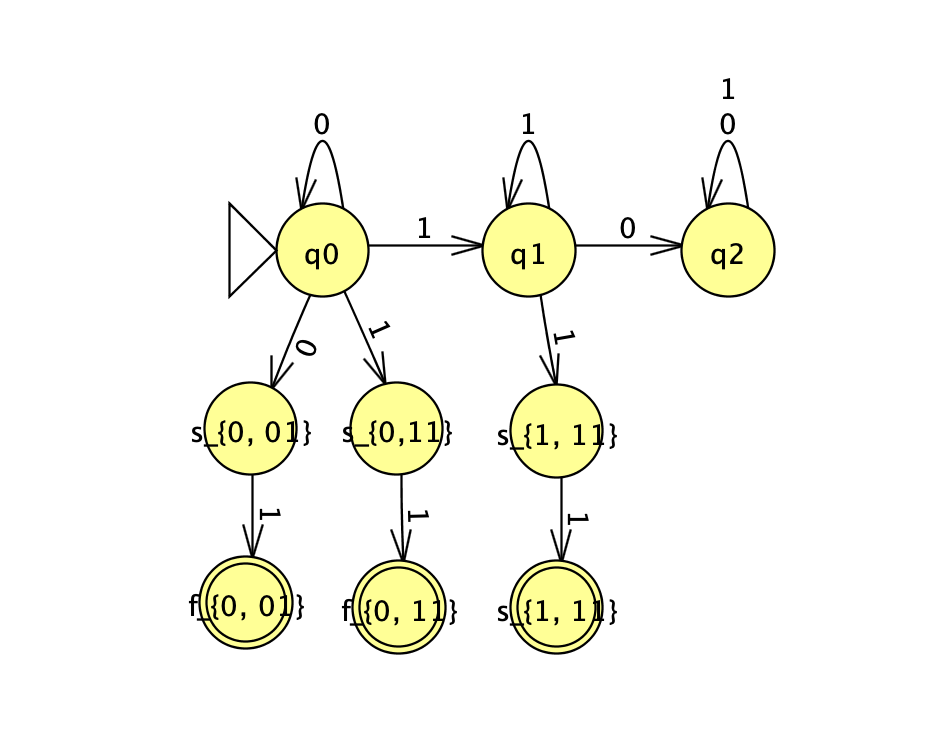
\includegraphics[width=75mm,scale=0.1]{a10.png}

\end{solution}

\item
\begin{question}
Prove that $L(M') = R3Last(L(M))$ for any deterministic finite automaton $M$ with input alphabet $\{0,1\}$.
\end{question}

\begin{solution}
{\bf Definintion:}\\
- $D$: The set of all DFAs with input alphabet $\{0,1\}$ \\
- ${\rm State}(M, s): D\times \{0,1\}^* \rightarrow Q = $ ``The state that the DFA $M$ will be in after it has parsed the string $s$'' \\
- ${\rm PATHS}(q_i, n): Q\times\nats\rightarrow Q^* $ = ``Set of every possible string of length $n$ that terminates at a final state starting at $q_i$''\\
{\bf Proof}:\\
\null\quad Let $M\in D$ be an arbitrary DFA\\
\null\qquad Let $s\in R3Last(L(M))$ be an arbitrary string\\
\null\qquad Therefore $\exists u,v\in \{0,1\}^*.(s = u\cdot v)$ (by $R3Last$ definition)\\
\null\qquad $\exists r\in\{0,1\}.[(urv\in L(M))\And (v\in\{0,1\}^2)]$ (by $R3Last$ definition)\\
\null\qquad $r\in\{0,1\}$ (by definition)\\
\null\qquad $v\in\{0,1\}^2$ (use of conjunction)\\
\null\qquad Therefore $|r| = 1$, $|v| = 2$ and $|r\cdot v| = 3$\\
\null\qquad Let $q_u = {\rm State}(M, u)$\\
\null\qquad By the definition of $Q'$ above, $q_u\in Q'$.\\
\null\qquad By the definition of $\delta'$ every path in $M$ is preserved, $q_u$ can be reached with the string $u$\\
\null\qquad Since $u\cdot r\cdot v \in L(M)$, $r\cdot v \in \rm PATHS(q_u,3)$ (by ${\rm PATHS}$ definition)\\
\null\qquad Therefore $v \in V_u$ (by $V_i$ definition)\\
\null\qquad By the definition of $\delta'$, and since $v\in V_u$ $s_{u, v} \in \delta'(q_u, v[1])$\\
\null\qquad By the definition of $\delta'$, and since $v\in V_u$ $f_{u,v} \in\delta' (s_{u,v}, v[2])$\\
\null\qquad Therefore there is a path from $q_u$ to $f_{u,v}$ with the two transitions $v[1]$ and $v[2]$\\
\null\qquad Since the string supplied to get to $q_u$ was $u$ and since the next two characters are $v[1]$\\
\null\qquad and $v[2]$. The string will be of the form $u\cdot v$.\\
\null\qquad Therefore since $f_{u,v}$ is a final state, $u\cdot v\in L(M')$\\
\null\qquad $s\in R3Last(L(M)) \And s = u\cdot v\And u\cdot v \in L(M')$ (proof of conjunction)\\
\null\qquad $s\in L(M')$\\
\null\quad $\forall s\in  R3Last(L(M)).(s\in L(M'))$ (generalization)\\
\null\quad $R3Last(L(M))\subseteq L(M')$ (subset proof)\\
\null\qquad Let $s\in L(M')$ be an arbitrary string\\
\null\qquad Since $s\in L(M')$ and by $F'$ definition, $\exists f_{i,v}\in F'.({\rm State}(M', s) = f_{i,v})$\\
\null\qquad By $\delta'$ definition, there is only one transition to $f_{i,v}$ from $s_{i,v}$ with the character $v[2]$\\
\null\qquad By $\delta'$ definition, there is only one transition to $s_{i,v}$ from $q_{i}$ with the character $v[1]$\\
\null\qquad Therefore the last two characters of $s$ are $v[1]$ and $v[2]$\\
\null\qquad Let $u$ be a string that when input into $M'$ can end up at state $q_u$\\
\null\qquad By the definition of $\delta'$ since $q_u\in Q$, the path to $q_u$ in $M'$ is the same as $M$ (no additional \\
\null\qquad transitions into any state in $Q$ were defined). Therefore $s = \cdot v$\\
\null\qquad Therefore ${\rm State}(M, u) = q_u$.\\
\null\qquad By the definition of $V_u$, $\exists r\in \{0,1\}.(r\cdot v\in {\rm PATHS(q_u, 3)})$\\
\null\qquad Therefore $u\cdot r \cdot v \in L(M)$\\
\null\qquad By the definition of $R3Last$, $u\cdot v\in R3Last(L(M))$\\
\null\qquad $u\cdot v \in R3Last(L(M)) \And u\cdot v = s$\\
\null\qquad $s\in R3Last(L(M))$
\null\quad $\forall s\in L(M'). (s\in R3Last(L(M)))$ (generalization)\\
\null\quad $L(M')\subseteq R3Last(L(M))$ (subset proof)\\
\null\quad Since $L(M')\subseteq R3Last(L(M))\And R3Last(L(M))\subseteq L(M')$, $L(M') = R3Last(L(M))$
$\forall M\in D.(L(M') = R3Last(L(M)))$ (generalization)\\
\end{solution}

\item
\begin{question}
Prove that, if $L \subseteq \{0,1\}^*$ is a regular language, then $R3Last(L)$ is regular.
\end{question}

\begin{solution}
{\bf Definintions:}\\
Let $R$ represent the set of all regular expressions \\
Let $D$ represent the set of all DFAs with input alphabet $\{0,1\}$ \\
Let $F$ represent the set of all finite automata with input alphabet $\{0,1\}$ \\
{\bf Proof:}\\
\null\quad Let $K\subseteq \{0,1\}^*$ be arbitrary\\
\null\qquad Assume $\exists r_k\in R.(L(r_k) = K)$ (definition of regular language)\\
\null\qquad $\forall N\subseteq\Sigma^*.[\exists r\in R.(L(r) = N) \Iff (\exists M\in D.(L(r) = L(M)))]$ (axiom from class)\\
\null\qquad Therefore let $M_k$ be a DFA such that $(L(r_k) = L(M_k))$\\
\null\qquad $(L(M_k) = L(r_k)) \And (L(R_k) = K)$ (proof of conjunction)\\
\null\qquad $L(M_k) = K$\\
\null\qquad As previously shown in pt 4, $\forall M\in D.(L(M') = R3Last(L(M)))$\\
\null\qquad Therefore let $M'_k$ be a finite automata such that $(L(M_k') = R3Last(L(M_k)))$\\
\null\qquad $\forall M\in F.\exists r\in R.(L(r) = L(M))$ (axiom from class)\\
\null\qquad\quad Choose $r'_k$ to be a regular expression such that $L(M_k') = L(r'_k)$\\
\null\qquad\quad $L(M_k') = R3Last(L(M_k))\And L(M_k') = L(r'_k)$ (proof of conjunction)\\
\null\qquad\quad $L(r'_k) = R3Last(L(M_k))$\\
\null\qquad\quad $L(M_k) = K \And L(r'_k) = R3Last(L(M_k))$ (proof of conjunction)\\
\null\qquad\quad $L(r'_k) = R3Last(K)$\\
\null\qquad $\exists r'_k\in R.(L(r'_k) = R3Last(k))$ (construction)\\
\null\quad $[\exists r_k\in R.(L(r_k) = K)]\Implies [\exists r'_k\in R.(L(r'_k) = R3Last(K))]$ \\
\null\quad (direct proof of implication)\\
$\forall K\subseteq \{0,1\}^*.[\exists r_k\in R.(L(r_k) = K)]\Implies [\exists r'_k\in R.(L(r'_k) = R3Last(K))]$ \\
(generalization)\\
Therefore for any language $L\subseteq \{0,1\}^*$, if that language is regular, $R3Last(K)$ is regular.\\
\end{solution}

\end{enumerate}
\end{document}
